\section{Fourier级数}
\label{sec:fourier-series}

在$\mathbb R^n$中取一组标准正交基$q_1,\ldots,q_n$，向量$v$的第$j$个坐标就是内积$a_j=\langle q_j,v\rangle$，并且$v=\sum_ja_jq_j$，$\lVert v\rVert^2=\sum_j\lvert a_j\rvert^2$。第~\ref{chap:function-inner-product-spaces}章把这套做法搬到了Hilbert空间。本节把它用在周期函数上，基取复指数$e^{\mathrm ikx}$，第$k$个基函数在一个周期内恰好转$k$圈，所以坐标记录的是第$k$次振荡的强弱。

先在$L^2$中建立展开，这是类比最直接的部分。然后问部分和在每一点、或在整个周期上一致地趋于什么，这两个问题要用到正交性之外的条件。

\subsection{\texorpdfstring{$L^2$}{L2}中的Fourier展开}
\label{sec:fourier-series-l2}

\paragraph{周期函数与归一化内积}

本节的函数都以$2\pi$为周期。等价地，可以把它看成区间$[-\pi,\pi)$上的函数，并把两个端点粘成一点。记这样的周期区间为$\mathbb T$，积分都在一个周期上进行。平方可积的周期函数组成$L^2(\mathbb T)$，它的元素是几乎处处相等的函数组成的等价类，第~\ref{chap:function-inner-product-spaces}章已证明它是Hilbert空间。

沿用第~\ref{chap:function-inner-product-spaces}章的约定，内积对第二个变量线性。我们在内积前放一个因子$1/(2\pi)$，使常数函数$1$的长度恰好为$1$：
\begin{equation}
\langle f,g\rangle=\frac1{2\pi}\int_{-\pi}^{\pi}\overline{f(x)}\,g(x)\,\mathrm dx .
\label{eq:fourier-circle-inner-product}
\end{equation}
相应的范数是$\lVert f\rVert_2=\langle f,f\rangle^{1/2}$。同样地，$L^1$范数也取平均：
\[
\lVert f\rVert_1=\frac1{2\pi}\int_{-\pi}^{\pi}\lvert f(x)\rvert\,\mathrm dx.
\]

记$e_k(x)=e^{\mathrm ikx}$，$k\in\mathbb Z$。下面验证它们标准正交。当$k=j$时，被积函数恒为$1$，所以$\langle e_j,e_k\rangle=1$。当$k\neq j$时，令$m=k-j\neq0$，直接积分得到
\[
\langle e_j,e_k\rangle=\frac1{2\pi}\int_{-\pi}^{\pi}e^{\mathrm imx}\,\mathrm dx
=\frac{e^{\mathrm im\pi}-e^{-\mathrm im\pi}}{2\pi\mathrm im}.
\]
由于$e^{\mathrm imx}$以$2\pi$为周期，分子中两个端点的值相同，所以
\[
\langle e_j,e_k\rangle=0.
\]
这正是周期性的作用：一个整数圈的旋转，正负部分恰好抵消。

\paragraph{Fourier系数与部分和}

有了标准正交系，第$k$个坐标自然就是与$e_k$的内积。

\begin{definition}[Fourier系数与Fourier级数]
\label{def:fourier-coefficients}
对$f\in L^1(\mathbb T)$，称
\begin{equation}
\widehat f(k)=\frac1{2\pi}\int_{-\pi}^{\pi}f(x)e^{-\mathrm ikx}\,\mathrm dx ,\qquad k\in\mathbb Z
\label{eq:fourier-coefficient}
\end{equation}
为$f$在方向$e_k$上的坐标，称为第$k$个\term{Fourier系数}（Fourier coefficient）。形式级数$\sum_{k\in\mathbb Z}\widehat f(k)e^{\mathrm ikx}$称为$f$的\term{Fourier级数}（Fourier series），它的对称部分和记为
\begin{equation}
S_Nf=\sum_{\lvert k\rvert\leq N}\widehat f(k)\,e_k .
\label{eq:fourier-partial-sum}
\end{equation}
\end{definition}

对$f\in L^2(\mathbb T)$，式~\eqref{eq:fourier-coefficient}就是$\widehat f(k)=\langle e_k,f\rangle$。只要$f$可积，系数就有定义，并且$\lvert\widehat f(k)\rvert\leq\lVert f\rVert_1$。一个周期的长度有限，由Cauchy--Schwarz不等式，$L^2(\mathbb T)\subseteq L^1(\mathbb T)$，所以平方可积函数都有系数。

于是一个函数对应一列坐标$[\ldots,\widehat f(-1),\widehat f(0),\widehat f(1),\ldots]$。下面算一个完整的例子，后面的定理都会回到它。

\begin{example}[方波的坐标]
\label{ex:fourier-square-wave}
取方波：在$(0,\pi)$上$f=1$，在$(-\pi,0)$上$f=-1$，再按$2\pi$周期延拓；在$0$和$\pm\pi$处的取值暂不规定。

$f$是奇函数，所以$\widehat f(0)=0$。对$k\neq0$，把积分分成两段：
\[
\widehat f(k)=\frac1{2\pi}\Bigl(\int_0^{\pi}e^{-\mathrm ikx}\,\mathrm dx-\int_{-\pi}^0e^{-\mathrm ikx}\,\mathrm dx\Bigr).
\]
两段分别积分，并用$e^{\pm\mathrm ik\pi}=(-1)^k$，得到
\[
\int_0^{\pi}e^{-\mathrm ikx}\,\mathrm dx=\frac{1-(-1)^k}{\mathrm ik},\qquad
\int_{-\pi}^0e^{-\mathrm ikx}\,\mathrm dx=\frac{(-1)^k-1}{\mathrm ik}.
\]
代回去，第$k$个系数是
\[
\widehat f(k)=\frac{1-(-1)^k}{\pi\mathrm ik}.
\]
偶数$k$的系数为零，奇数$k$的系数为$2/(\pi\mathrm ik)$，模长为$2/(\pi\lvert k\rvert)$。

把$\pm k$两项配对，括号里出现$2\mathrm i\sin kx$，得到第$k$次（$k$为正奇数）的实形式
\[
\widehat f(k)e^{\mathrm ikx}+\widehat f(-k)e^{-\mathrm ikx}=\frac4{\pi k}\sin kx.
\]
所以前几项是
\[
S_5f(x)=\frac4\pi\Bigl(\sin x+\frac13\sin3x+\frac15\sin5x\Bigr).
\]
\end{example}

图~\ref{fig:fourier-square-coordinates}把这个例子的两种“一列数”并排放在一起。左边是取值，下标是$x$；右边是坐标，下标是$k$。同一个向量换了一组基来记录，三条灰色的正弦波叠加起来，已经勾出方波的轮廓。

\begin{BookInlineFigure}
  \centering
  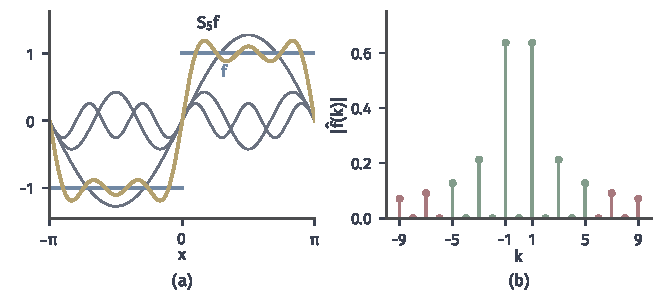
\includegraphics[width=112mm]{figures/04-spaces-measures-and-geometry/03-function-spaces/matplotlib/fourier-square-coordinates/figure.pdf}
  \caption{方波的两种记录方式。(a)蓝色为方波$f$，灰色为$\frac4{\pi}\sin x$、$\frac4{3\pi}\sin3x$、$\frac4{5\pi}\sin5x$三个分量，黄色为它们的和$S_5f$。(b)模长$\lvert\widehat f(k)\rvert$，绿色为$S_5f$保留的坐标（$\lvert k\rvert\leq5$），红色为舍弃的坐标；偶数下标的坐标都是零。}
  \label{fig:fourier-square-coordinates}
\end{BookInlineFigure}

部分和有明确的几何含义。有限组合$\sum_{\lvert k\rvert\leq N}c_ke_k$称为次数不超过$N$的\term{三角多项式}（trigonometric polynomial），它们组成$2N+1$维子空间$\mathcal T_N$。由第~\ref{chap:function-inner-product-spaces}章的有限截断定理，$S_Nf$是$f$在$\mathcal T_N$上的正交投影，也就是$\mathcal T_N$中离$f$最近的元素。同一章的Bessel不等式给出
\[
\sum_{k\in\mathbb Z}\lvert\widehat f(k)\rvert^2\leq\lVert f\rVert_2^2 .
\]

表~\ref{tab:fourier-dictionary}汇总了目前的对应。最后一行是类比失效的地方。

\begin{BookInlineTable}
  \centering
  \begin{tabular}{@{}ll@{}}
    \toprule
    $\mathbb C^n$与标准正交基$q_j$ & $L^2(\mathbb T)$与$e_k=e^{\mathrm ikx}$\\
    \midrule
    坐标$a_j=\langle q_j,v\rangle$ & Fourier系数$\widehat f(k)=\langle e_k,f\rangle$\\
    投影到前几个基向量 & 部分和$S_Nf$\\
    $\sum_j\lvert a_j\rvert^2\leq\lVert v\rVert^2$ & Bessel不等式\\
    $v=\sum_ja_jq_j$，有限和 & $f=\sum_k\widehat f(k)e_k$，$L^2$收敛\\
    $n$个正交向量自动成基 & 无穷多个正交元素未必成基\\
    \bottomrule
  \end{tabular}
  \caption{有限维标准正交基与复指数系的对应。}
  \label{tab:fourier-dictionary}
\end{BookInlineTable}

有限维中，$n$个标准正交向量必定张成全空间。无限维中，数量不能说明问题：从$\{e_k\}$中拿掉$e_0$，剩下的仍是无穷多个标准正交元素，但常数函数$1$与它们全部正交，再也表示不出来。所以写“级数”时还没有断言它收敛，更没有断言它等于$f$。要得到$L^2$中的等式，还需要证明这个系是完备的：与所有$e_k$正交的元素只有零。

\paragraph{Fejér平均}

要证明完备性，一种办法是把$f$写成三角多项式的极限，而这些三角多项式只依赖于$f$的Fourier系数。这样，系数全为零的函数就只能是零。先试部分和$S_Nf$本身。把系数的定义代入式~\eqref{eq:fourier-partial-sum}，交换有限和与积分，再利用周期函数平移不改变一个周期上的积分，得到
\begin{equation}
S_Nf(x)=\frac1{2\pi}\int_{-\pi}^{\pi}f(x-t)D_N(t)\,\mathrm dt ,
\label{eq:fourier-dirichlet-integral}
\end{equation}
其中
\[
D_N(t)=\sum_{\lvert k\rvert\leq N}e^{\mathrm ikt}
\]
称为\term{Dirichlet核}（Dirichlet kernel）。

$D_N$有闭式。当$t\notin2\pi\mathbb Z$时，这是一个公比为$e^{\mathrm it}$的几何级数，首项为$e^{-\mathrm iNt}$，共$2N+1$项：
\[
D_N(t)=e^{-\mathrm iNt}\,\frac{e^{\mathrm i(2N+1)t}-1}{e^{\mathrm it}-1}.
\]
分子分母同乘$e^{-\mathrm it/2}$，分母变成$2\mathrm i\sin(t/2)$，分子变成$2\mathrm i\sin\bigl((N+\tfrac12)t\bigr)$乘同一个相位，相位恰好抵消。于是
\begin{equation}
D_N(t)=\frac{\sin\bigl((N+\tfrac12)t\bigr)}{\sin(t/2)} .
\label{eq:fourier-dirichlet-closed}
\end{equation}

式~\eqref{eq:fourier-dirichlet-integral}是$f$的一种加权平均，但$D_N$的权有正有负。图~\ref{fig:fourier-kernels}(a)是$N=8$的情形，中央峰高$2N+1=17$，两侧的振荡并不随$N$增大而变小，这使得直接估计$S_Nf-f$很困难。

补救办法是取部分和的算术平均。令
\[
\sigma_Nf=\frac1{N+1}\sum_{n=0}^{N}S_nf,
\]
它对应的核是$F_N=\frac1{N+1}\sum_{n=0}^ND_n$，称为\term{Fejér核}（Fejér kernel）。这相当于把振荡的正负部分在不同的$n$之间相互抵消。

下面算$F_N$的闭式。由式~\eqref{eq:fourier-dirichlet-closed}，分子分母都乘$\sin(t/2)$，并用积化和差公式
\[
\sin\bigl((n+\tfrac12)t\bigr)\sin(t/2)=\tfrac12\bigl(\cos nt-\cos(n+1)t\bigr).
\]
对$n=0,\ldots,N$求和时中间项相消，只剩$\tfrac12\bigl(1-\cos(N+1)t\bigr)$，所以
\[
F_N(t)=\frac1{N+1}\,\frac{1-\cos\bigl((N+1)t\bigr)}{2\sin^2(t/2)}.
\]
再用$1-\cos\theta=2\sin^2(\theta/2)$，得到
\begin{equation}
F_N(t)=\frac1{N+1}\Bigl(\frac{\sin\bigl((N+1)t/2\bigr)}{\sin(t/2)}\Bigr)^2 .
\label{eq:fourier-fejer-closed}
\end{equation}

\begin{BookInlineFigure}
  \centering
  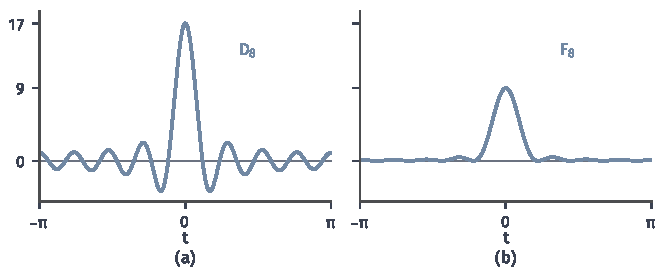
\includegraphics[width=112mm]{figures/04-spaces-measures-and-geometry/03-function-spaces/matplotlib/fourier-kernels/figure.pdf}
  \caption{$N=8$时的两个核，纵轴相同。(a)Dirichlet核$D_8$在$t=0$处高$17$，两侧正负交替。(b)Fejér核$F_8$在$t=0$处高$9$，处处非负，远离原点时几乎为零。}
  \label{fig:fourier-kernels}
\end{BookInlineFigure}

$F_N$有三条性质，恰好是把它当作“集中于原点的权”所需要的，图~\ref{fig:fourier-kernels}(b)可以对照：
\begin{itemize}
\item $F_N\geq0$，这从式~\eqref{eq:fourier-fejer-closed}直接读出；
\item $\frac1{2\pi}\int_{-\pi}^{\pi}F_N=1$，因为每个$D_n$只有常数项$1$对积分有贡献；
\item 对$0<\delta\leq\lvert t\rvert\leq\pi$，$F_N(t)\leq\dfrac1{(N+1)\sin^2(\delta/2)}$，所以质量随$N$增大集中到原点附近。
\end{itemize}

\begin{lemma}[Fejér平均的收敛]
\label{lem:fourier-fejer}
若$f$是连续的周期函数，则$\sigma_Nf$一致收敛到$f$。若$f\in L^2(\mathbb T)$，则$\lVert\sigma_Nf-f\rVert_2\to0$。
\end{lemma}

\begin{proof}
由$F_N$的积分为$1$，把$f(x)$写进积分，得到
\[
\sigma_Nf(x)-f(x)=\frac1{2\pi}\int_{-\pi}^{\pi}\bigl(f(x-t)-f(x)\bigr)F_N(t)\,\mathrm dt.
\]

先看连续的$f$。它在紧区间上一致连续，记
\[
\omega(\delta)=\sup_{\lvert t\rvert<\delta}\sup_x\lvert f(x-t)-f(x)\rvert,
\]
则$\delta\to0$时$\omega(\delta)\to0$。把积分分成$\lvert t\rvert<\delta$与$\delta\leq\lvert t\rvert\leq\pi$两部分。前一部分用$\omega(\delta)$控制差、用积分为$1$控制权；后一部分把差的绝对值放大为$2\lVert f\rVert_\infty$，再用$F_N$的第三条性质。于是
\[
\lvert\sigma_Nf(x)-f(x)\rvert\leq\omega(\delta)+\frac{2\lVert f\rVert_\infty}{(N+1)\sin^2(\delta/2)}.
\]
右边与$x$无关。先取$\delta$使第一项小，再令$N$充分大使第二项小，即得一致收敛。

再看$f\in L^2(\mathbb T)$。由前两条性质，$\frac1{2\pi}F_N(t)\,\mathrm dt$是一个周期上的概率测度。对它用Cauchy--Schwarz不等式，得到
\[
\lvert\sigma_Nf(x)-f(x)\rvert^2\leq\frac1{2\pi}\int_{-\pi}^{\pi}\lvert f(x-t)-f(x)\rvert^2F_N(t)\,\mathrm dt.
\]
对$x$按归一化测度积分，并用Tonelli定理交换次序。记平移$(\tau_tf)(x)=f(x-t)$，于是
\[
\lVert\sigma_Nf-f\rVert_2^2\leq\frac1{2\pi}\int_{-\pi}^{\pi}\lVert\tau_tf-f\rVert_2^2\,F_N(t)\,\mathrm dt.
\]
同样分成$\lvert t\rvert<\delta$与其余部分，并用$\lVert\tau_tf-f\rVert_2\leq2\lVert f\rVert_2$。这样只需再说明$t\to0$时$\lVert\tau_tf-f\rVert_2\to0$。

这一平移连续性分三步得到。第~\ref{chap:smoothing-weak-derivatives}章证明了$\mathbb R$上的可积函数$F$满足$\int\lvert F(x-h)-F(x)\rvert\,\mathrm dx\to0$。对周期函数$f$与$\lvert h\rvert\leq\pi$，取$F=f\mathbf 1_{[-2\pi,2\pi]}$，在$x\in[-\pi,\pi]$上$F(x-h)=f(x-h)$，所以周期情形的$L^1$平移连续性成立。

若还有$\lvert f\rvert\leq n$，则
\[
\lvert\tau_hf-f\rvert^2\leq2n\,\lvert\tau_hf-f\rvert,
\]
所以有界函数的$L^2$平移连续性成立。

对一般的$f\in L^2(\mathbb T)$，取$f_n=f\mathbf 1_{\{\lvert f\rvert\leq n\}}$。由控制收敛定理，$\lVert f-f_n\rVert_2\to0$。平移不改变周期函数的范数，所以
\[
\lVert\tau_hf-f\rVert_2\leq2\lVert f-f_n\rVert_2+\lVert\tau_hf_n-f_n\rVert_2.
\]
先取$n$使第一项小，再令$h\to0$，第二项趋于零。
\end{proof}

\paragraph{完备性与Parseval关系}

$\sigma_Nf$完全由Fourier系数决定，这正是证明完备性所需要的。

\begin{theorem}[$L^2$中的Fourier展开]
\label{thm:fourier-series-l2}
$\{e_k\}_{k\in\mathbb Z}$是$L^2(\mathbb T)$的完备标准正交系。因此对每个$f\in L^2(\mathbb T)$，$\lVert S_Nf-f\rVert_2\to0$，并且
\begin{equation}
\begin{gathered}
\frac1{2\pi}\int_{-\pi}^{\pi}\lvert f(x)\rvert^2\,\mathrm dx=\sum_{k\in\mathbb Z}\lvert\widehat f(k)\rvert^2 ,\\
\langle f,g\rangle=\sum_{k\in\mathbb Z}\overline{\widehat f(k)}\,\widehat g(k) .
\end{gathered}
\label{eq:fourier-series-parseval}
\end{equation}
\end{theorem}

\begin{proof}
设$f\in L^2(\mathbb T)$与每个$e_k$正交，即全部$\widehat f(k)=0$。则每个$S_nf=0$，从而$\sigma_Nf=0$。由引理~\ref{lem:fourier-fejer}，$\sigma_Nf\to f$于$L^2$，所以$f=0$。完备标准正交系的范数收敛展开、Parseval等式及内积公式，由第~\ref{chap:function-inner-product-spaces}章的正交展开定理给出。
\end{proof}

式~\eqref{eq:fourier-series-parseval}就是无限维的勾股定理：一个周期上的平均能量等于各坐标模平方之和，本章称为Parseval关系。截断误差也由它读出，投影与残差正交，所以
\begin{equation}
\lVert f-S_Nf\rVert_2^2=\sum_{\lvert k\rvert>N}\lvert\widehat f(k)\rvert^2 .
\label{eq:fourier-series-truncation}
\end{equation}

结合第~\ref{chap:function-inner-product-spaces}章的结论，$f\mapsto(\widehat f(k))_{k\in\mathbb Z}$是$L^2(\mathbb T)$到$\ell^2(\mathbb Z)$的保持内积的双射。在$L^2$的意义下，“函数是一列坐标”这句话是严格成立的。

用方波核对一下。左边的平均能量为$1$，右边只有奇数$k$有贡献，每个模平方为$4/(\pi^2k^2)$，$\pm k$各一项，所以
\[
1=2\sum_{j\geq0}\frac{4}{\pi^2(2j+1)^2}.
\]
整理后得到一个级数的值：
\[
\sum_{j\geq0}\frac1{(2j+1)^2}=\frac{\pi^2}8 .
\]

截断误差也可以逐项算出。前几项的平方和分别是
\[
\frac8{\pi^2}\approx0.8106,\qquad
\frac8{\pi^2}\Bigl(1+\frac19\Bigr)\approx0.9006,\qquad
\frac8{\pi^2}\Bigl(1+\frac19+\frac1{25}\Bigr)\approx0.9331.
\]
由式~\eqref{eq:fourier-series-truncation}，$\lVert f-S_Nf\rVert_2^2$在$N=1,3,5$时分别约为$0.1894$、$0.0994$、$0.0669$。每增加一个坐标，误差平方恰好减少该坐标的模平方，已经算好的系数不必修改，这是正交基的好处。系数的衰减怎样决定误差的速度，留到第~\ref{chap:function-approximation}章研究。

\paragraph{实形式与一般周期}

实值函数也常用正弦与余弦展开。若$f$为实值，对式~\eqref{eq:fourier-coefficient}取共轭得到$\widehat f(-k)=\overline{\widehat f(k)}$。把$\pm k$两项配对，就得到实形式：
\[
f\sim\frac{a_0}2+\sum_{k\geq1}\bigl(a_k\cos kx+b_k\sin kx\bigr),
\]
其中
\[
a_k=\frac1\pi\int_{-\pi}^{\pi}f(x)\cos kx\,\mathrm dx,\qquad
b_k=\frac1\pi\int_{-\pi}^{\pi}f(x)\sin kx\,\mathrm dx.
\]
两套系数的关系是
\[
\widehat f(0)=\frac{a_0}2,\qquad\widehat f(k)=\frac{a_k-\mathrm ib_k}2\quad(k\geq1).
\]
相应地，Parseval关系写成
\[
\frac1{2\pi}\int_{-\pi}^{\pi}\lvert f\rvert^2=\frac{a_0^2}4+\frac12\sum_{k\geq1}(a_k^2+b_k^2).
\]

两种写法表示同一个展开，实形式中的$1/\pi$与$1/2$都来自配对。方波的实系数是$a_k=0$，奇数$k$时$b_k=4/(\pi k)$，与例~\ref{ex:fourier-square-wave}一致。这相当于把同一组坐标换成实的基$1,\sqrt2\cos kx,\sqrt2\sin kx$来写，只是常数放的位置不同。

若周期是$T$而不是$2\pi$，令$x=2\pi t/T$即可化归本节情形。这时系数为
\begin{equation}
c_k=\frac1T\int_0^Tf(t)\,e^{-2\pi\mathrm ikt/T}\,\mathrm dt ,
\label{eq:fourier-period-T}
\end{equation}
第$k$个基函数的频率是单位长度内$k/T$圈。周期越长，相邻频率越靠近，这一点在下一节开头会用到。

\paragraph{系数描述的是等价类}

类比还有一个需要注意的地方。Fourier系数是积分，改变$f$在一个零测集上的值不改变任何坐标。所以坐标记录的不是一张逐点的取值表，而是$L^2(\mathbb T)$中的一个等价类。定理~\ref{thm:fourier-series-l2}中的展开是范数意义下的等式，不是逐点等式。

例~\ref{ex:fourier-square-wave}中没有规定方波在$0$和$\pm\pi$处的取值，原因就在这里：无论在这些点赋什么值，算出来的系数都一样，$\pi^2/8$这个结果也一样。要讨论$S_Nf$在某一点的值，必须另外加条件，这是下一小节的内容。

\subsection{点态收敛}
\label{sec:fourier-series-pointwise}

$L^2$收敛控制的是一个周期上的平均平方误差，它不告诉我们部分和在某个给定点处是否收敛。连续性也不够：du Bois-Reymond构造过连续周期函数，其Fourier级数在某一点发散，构造较长，读者可查阅Fourier分析的教材。所以逐点结论必须对$f$加上比连续更强的局部条件，本小节使用分段$C^1$条件。

\paragraph{Riemann--Lebesgue引理}

逐点收敛的证明最终要说明一个高频振荡积分趋于零。直观上，$g(t)e^{-\mathrm i\lambda t}$在长度为$\pi/\lambda$的小段上一正一负，而$g$在这么短的距离上几乎不变，正负两部分几乎抵消。这件事对任何可积函数都成立。

\begin{lemma}[Riemann--Lebesgue引理]
\label{lem:fourier-riemann-lebesgue}
若$g\in L^1(\mathbb R)$，则$\lvert\lambda\rvert\to\infty$时
\begin{equation}
\int_{\mathbb R}g(t)e^{-\mathrm i\lambda t}\,\mathrm dt\to0 .
\label{eq:fourier-riemann-lebesgue}
\end{equation}
特别地，$\int g(t)\sin(\lambda t)\,\mathrm dt\to0$；对$f\in L^1(\mathbb T)$，$\lvert k\rvert\to\infty$时$\widehat f(k)\to0$。
\end{lemma}

\begin{proof}
把式~\eqref{eq:fourier-riemann-lebesgue}左边的积分记为$I(\lambda)$，$\lambda\neq0$。作换元$t\mapsto t+\pi/\lambda$，并用$e^{-\mathrm i\pi}=-1$，得到
\[
I(\lambda)=-\int_{\mathbb R}g(t+\pi/\lambda)\,e^{-\mathrm i\lambda t}\,\mathrm dt.
\]
把它与原式相加再取模，得到
\[
2\lvert I(\lambda)\rvert\leq\int_{\mathbb R}\lvert g(t)-g(t+\pi/\lambda)\rvert\,\mathrm dt.
\]
由第~\ref{chap:smoothing-weak-derivatives}章的平移积分连续性，右边在$\lvert\lambda\rvert\to\infty$时趋于零。对$\lambda$取实部虚部即得正弦情形。周期情形把$f$在一个周期外置零，再取$\lambda=k$。
\end{proof}

对$L^2$函数，坐标趋于零可以由Bessel不等式读出，因为平方可和的序列必趋于零。引理的新内容在于它只要求可积，而$L^1(\mathbb T)$函数的坐标不必平方可和。它也不给出趋于零的速度：方波的系数按$1/\lvert k\rvert$衰减，后面会看到更光滑的函数衰减得更快。

\paragraph{分段$C^1$函数的Dirichlet定理}

称周期函数$f$为分段$C^1$，是指在一个周期$[-\pi,\pi]$中有有限个分点，使$f$在每个开子区间上连续可微，并且$f$与$f'$在每个子区间端点处有单侧极限。于是在每一点$x$都存在单侧极限$f(x+)$与$f(x-)$，它们在连续点相等，在跳跃点不等。方波是最典型的例子。

\begin{theorem}[Dirichlet定理]
\label{thm:fourier-dirichlet}
设$f$是分段$C^1$的$2\pi$周期函数，则对每个$x\in\mathbb R$，
\begin{equation}
\lim_{N\to\infty}S_Nf(x)=\frac{f(x+)+f(x-)}2 .
\label{eq:fourier-dirichlet-limit}
\end{equation}
特别地，在$f$的连续点，$S_Nf(x)\to f(x)$。
\end{theorem}

\begin{proof}
$D_N$是偶函数，所以式~\eqref{eq:fourier-dirichlet-integral}可以按$t>0$与$t<0$合并为
\[
S_Nf(x)=\frac1{2\pi}\int_0^{\pi}\bigl[f(x+t)+f(x-t)\bigr]D_N(t)\,\mathrm dt.
\]
又由$D_N$的积分得$\frac1{2\pi}\int_0^{\pi}D_N=\frac12$，因此可以把左右极限的平均写进同一个积分。记
\[
h(t)=f(x+t)-f(x+)+f(x-t)-f(x-),
\]
并利用式~\eqref{eq:fourier-dirichlet-closed}，得到
\[
S_Nf(x)-\frac{f(x+)+f(x-)}2=\frac1{2\pi}\int_0^{\pi}\frac{h(t)}{\sin(t/2)}\sin\bigl((N+\tfrac12)t\bigr)\,\mathrm dt.
\]
只需说明$g(t)=h(t)/\sin(t/2)$在$(0,\pi)$上可积，然后对$g\mathbf 1_{(0,\pi)}$用引理~\ref{lem:fourier-riemann-lebesgue}。

取$t_0>0$，小于$x$到两侧最近分点的距离。在$(x,x+t_0)$上$f$连续可微，$f'$有单侧极限，所以$\lvert f'\rvert\leq C$。对$0<s<t<t_0$用中值定理，得到$\lvert f(x+t)-f(x+s)\rvert\leq C(t-s)$。令$s\to0^+$，得到
\[
\lvert f(x+t)-f(x+)\rvert\leq Ct.
\]
左侧同理。又$0\leq t\leq\pi$时$\sin(t/2)\geq t/\pi$，所以$g$在$(0,t_0)$上有界。在$[t_0,\pi]$上，$\sin(t/2)\geq\sin(t_0/2)>0$，而$f$有界，$g$也有界。因此$g$可积，引理给出右边趋于零。
\end{proof}

\paragraph{连续点、跳跃点与等价类}

定理把每一点分成两类，用方波可以逐一核对。取连续点$x=\pi/2$，这时$\sin(k\pi/2)$对$k=1,3,5,\ldots$依次为$1,-1,1,\ldots$，所以
\[
S_Nf\Bigl(\frac\pi2\Bigr)=\frac4\pi\Bigl(1-\frac13+\frac15-\cdots\Bigr).
\]
$N=1,3,5,7$时的值依次约为$1.273$、$0.849$、$1.104$、$0.922$，在$f(\pi/2)=1$的两侧摆动着收敛。

再取跳跃点$x=0$。每个$\sin(k\cdot0)=0$，所以$S_Nf(0)=0$对一切$N$成立，这正是左右极限的平均$(1+(-1))/2$。无论在$0$处给方波赋什么值，极限都是$0$：单点赋值既不进入系数，也不进入单侧极限。

与$L^2$展开相比，这里多用了$x$两侧的单侧Lipschitz估计，它来自分段$C^1$假设，使$g$在$t=0$附近可积；Riemann--Lebesgue引理本身只需要可积性。证明还显示了收敛的局部性：$g$只在$x$附近需要特别的估计，远离$x$处只用了有界性。$L^2$收敛不能代替这里的局部条件，因为它允许在零测集上任意修改函数，而逐点问题恰恰关心单个点。

\subsection{一致收敛}
\label{sec:fourier-series-uniform}

点态收敛允许不同点以不同速度收敛，一致收敛则要求整个周期上的最大误差趋于零。一个简单的充分条件是坐标绝对可和，而坐标衰减的速度由函数的光滑性控制。

\paragraph{分部积分与系数衰减}

对连续可微的周期函数，分部积分把求导转到坐标上。在$\widehat{f'}(k)$的定义中分部积分，得到
\[
\widehat{f'}(k)=\frac1{2\pi}\Bigl[f(x)e^{-\mathrm ikx}\Bigr]_{-\pi}^{\pi}+\frac{\mathrm ik}{2\pi}\int_{-\pi}^{\pi}f(x)e^{-\mathrm ikx}\,\mathrm dx.
\]
$f$与$e^{-\mathrm ikx}$都以$2\pi$为周期，边界项为零，所以
\begin{equation}
\widehat{f'}(k)=\mathrm ik\,\widehat f(k).
\label{eq:fourier-series-derivative}
\end{equation}
求导在这组坐标下是对角矩阵$\operatorname{diag}(\mathrm ik)$。这一步依赖周期性：若$f(\pi)\neq f(-\pi)$，边界项不为零。

\begin{theorem}[$C^2$函数的一致收敛]
\label{thm:fourier-uniform}
设$f$是二次连续可微的$2\pi$周期函数。则对$k\neq0$有
\begin{equation}
\lvert\widehat f(k)\rvert\leq\frac{\lVert f''\rVert_\infty}{k^2},
\label{eq:fourier-c2-coefficient}
\end{equation}
$\sum_k\lvert\widehat f(k)\rvert<\infty$，并且$S_Nf$一致收敛到$f$，
\begin{equation}
\sup_x\lvert f(x)-S_Nf(x)\rvert\leq\frac{2\lVert f''\rVert_\infty}{N},\qquad N\geq1 .
\label{eq:fourier-c2-uniform-error}
\end{equation}
\end{theorem}

\begin{proof}
用式~\eqref{eq:fourier-series-derivative}两次，得到$\widehat{f''}(k)=-k^2\widehat f(k)$。而$\widehat{f''}(k)$的模不超过$\lVert f''\rVert_1\leq\lVert f''\rVert_\infty$，这给出系数估计。

由$\sum_{k\neq0}k^{-2}<\infty$，Weierstrass判别法说明$S_Nf$一致收敛到某个连续函数$h$。一致收敛蕴含$L^2$收敛，而定理~\ref{thm:fourier-series-l2}说明$S_Nf\to f$于$L^2$，所以$h=f$几乎处处。两个连续函数若在某点不等，就在该点的一个邻域内不等，邻域的测度为正，所以$h=f$处处成立。

误差估计来自尾部求和。对每个$x$，误差不超过被舍弃坐标的模之和：
\[
\lvert f(x)-S_Nf(x)\rvert\leq\sum_{\lvert k\rvert>N}\lvert\widehat f(k)\rvert.
\]
由式~\eqref{eq:fourier-c2-coefficient}，只需估计$k^{-2}$的尾部和：
\[
\sum_{\lvert k\rvert>N}\frac1{k^2}=2\sum_{k>N}\frac1{k^2}\leq2\int_N^\infty\frac{\mathrm dt}{t^2}=\frac2N.
\]
乘上$\lVert f''\rVert_\infty$，就是式~\eqref{eq:fourier-c2-uniform-error}。
\end{proof}

$C^2$只是一个方便的充分条件，连续可微就已足够。由式~\eqref{eq:fourier-series-derivative}与Cauchy--Schwarz不等式，
\[
\sum_{k\neq0}\lvert\widehat f(k)\rvert=\sum_{k\neq0}\frac{\lvert\widehat{f'}(k)\rvert}{\lvert k\rvert}
\leq\lVert f'\rVert_2\Bigl(\sum_{k\neq0}\frac1{k^2}\Bigr)^{1/2},
\]
这里用到$f'$的Parseval关系。

不必处处可导。周期延拓的$\lvert x\rvert$（三角波）在$0$与$\pm\pi$处有尖点，分部积分得到它的系数：
\[
\widehat f(0)=\frac\pi2,\qquad
\widehat f(k)=\frac{(-1)^k-1}{\pi k^2}\quad(k\neq0).
\]
奇数$k$时$\widehat f(k)=-2/(\pi k^2)$，偶数$k\neq0$时为零，绝对可和，所以部分和一致收敛，极限与$f$处处相等的论证同上。

在$x=0$处取值，右边是$\pi/2$减去正数项，得到
\[
0=\frac\pi2-\frac4\pi\sum_{j\geq0}\frac1{(2j+1)^2},
\]
这与方波的Parseval关系给出的$\pi^2/8$一致。逐项算，$N=1,3,5,9$时$S_Nf(0)$依次约为$0.298$、$0.156$、$0.105$、$0.064$，趋于$f(0)=0$。

比较两个例子。方波有跳跃，系数按$1/\lvert k\rvert$衰减，不绝对可和；三角波连续，只有尖点，系数按$1/k^2$衰减，绝对可和。函数越光滑，高频坐标越小。

\paragraph{三种误差的比较}

三种收敛方式衡量的是不同的误差。一致误差$\sup_x\lvert f-S_Nf\rvert$控制每一点，因而控制逐点误差。由$\lVert\cdot\rVert_2\leq\sup\lvert\cdot\rvert$，它也控制$L^2$误差。反过来，$L^2$误差小只说明误差大的地方测度小，逐点收敛也可以在不同点有不同速度。

跳跃函数不能获得一致收敛。部分和$S_Nf$是三角多项式，处处连续；一致收敛的连续函数列的极限连续，可参考\BookChapterRef{chap:limits-continuity}{卷一第5章“极限与连续”}。方波在$0$处跳跃，所以$S_Nf$不可能一致收敛到任何与方波几乎处处相等的函数。

具体的情形可以算出来。取$N=2n-1$，对$S_Nf$求导，用几何级数求和得
\[
(S_Nf)'(x)=\frac4\pi\sum_{j=1}^n\cos\bigl((2j-1)x\bigr)=\frac2\pi\cdot\frac{\sin 2nx}{\sin x}.
\]
所以在$x>0$一侧，第一个峰出现在$x=\pi/(2n)$。把这一点代入$S_Nf$，并记$x_j=(2j-1)\pi/(2n)$，有$\frac1{2j-1}=\frac{\pi}{2n\,x_j}$，于是
\[
S_Nf\Bigl(\frac\pi{2n}\Bigr)=\frac2\pi\sum_{j=1}^n\frac{\sin x_j}{x_j}\cdot\frac\pi n.
\]
右边是$\sin u/u$在$[0,\pi]$上步长$\pi/n$的中点Riemann和，所以$n\to\infty$时
\[
S_Nf\Bigl(\frac\pi{2n}\Bigr)\to\frac2\pi\int_0^\pi\frac{\sin u}{u}\,\mathrm du\approx1.179.
\]
这就是\term{Gibbs现象}（Gibbs phenomenon）：跳跃附近的部分和总要越过跳跃高度，超出约$0.179$，即跳跃幅度$2$的约$9\%$，而峰的位置随$N$增大向跳跃点收缩。$N=9,25,81$时峰值依次约为$1.182$、$1.180$、$1.179$。

\begin{BookInlineFigure}
  \centering
  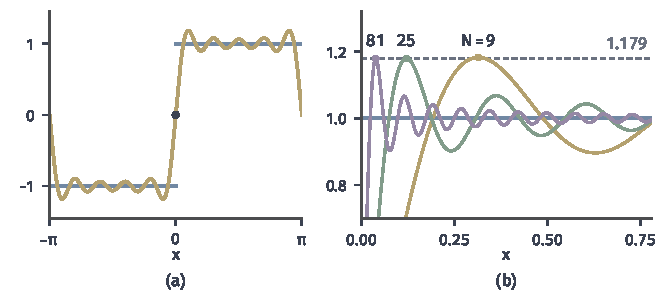
\includegraphics[width=112mm]{figures/04-spaces-measures-and-geometry/03-function-spaces/matplotlib/fourier-gibbs/figure.pdf}
  \caption{方波的Gibbs现象。蓝色为方波。(a)$N=9$的部分和（黄色），在跳跃点$0$处取值$0$（黑点）。(b)$x>0$一侧的放大图，黄、绿、紫分别为$N=9,25,81$，圆点是各自的第一个峰，都接近虚线$1.179$，峰随$N$增大靠近跳跃点。}
  \label{fig:fourier-gibbs}
\end{BookInlineFigure}

图~\ref{fig:fourier-gibbs}(b)说明这与定理~\ref{thm:fourier-dirichlet}并不矛盾。固定一个$x>0$，峰迟早越过它，之后$S_Nf(x)$趋于$1$；只是越靠近跳跃点，收敛越晚，所以最大误差始终不小。三种误差在方波上的表现是：$L^2$误差趋于零，每个固定点的误差趋于零，而一致误差不趋于零。
